\section{Design}\label{sec:design}

Below is a figure of the general architecture of our implementation at the end of Sprint 1, this is a more finalized version but will be updated during sprint 2 if necessary.
\begin{figure}[ht]
\centering
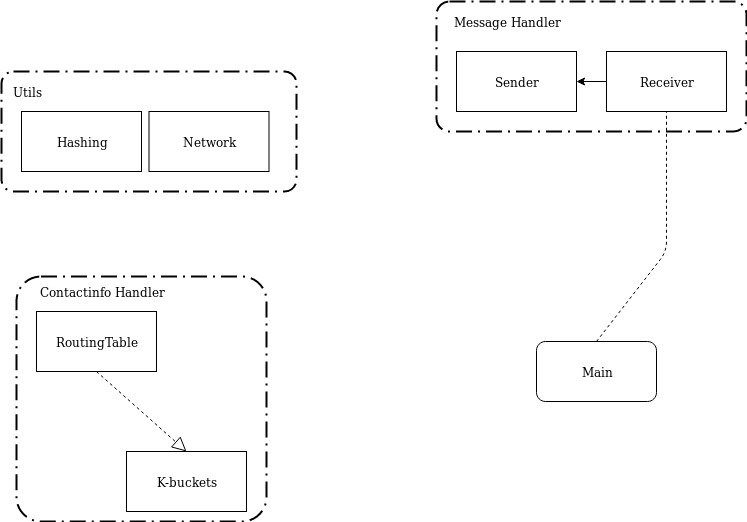
\includegraphics[width=\linewidth]{D7024E-architecture.jpg}
\caption{High-level architecture of a node in the kademlia implementation.}
\end{figure}

The main function starts a cliserver to handle incoming communication through a cliclient and starts a reciever. The reciever listens as the 'busy-wait' loop so that the node does not terminate but awaits further instructions. The receiver then spawns new threads (goroutines) as needed to handle incoming instructions. The sender is used to send any messages to other nodes in the network. Utils handles any general functions such as hashing, a node getting its own IP, etc. While the routing table keeps records of a nodes k-buckets.
The cliserver will always listen on its IP and port 80 for incoming connections from cliclients, the server is limited to handling one connection at the time. Any commands from the cliclient that effects the kademlia network goes through an API. We chose this API as an access point as we plan to implement rest API in sprint 2.

